\documentclass[type = bachelor]{whu-thesis}
% \documentclass[type = master]{whu-thesis}
% \documentclass[type = doctor]{whu-thesis}
% \documentclass[type = master,showframe]{whu-thesis}
% \documentclass[type = doctor,showframe]{whu-thesis}
% \documentclass[type = bachelor,showframe]{whu-thesis}\small
\usepackage{caption}
\usepackage{subcaption}
\usepackage{listings}
\usepackage{graphicx}
\usepackage{algorithm2e}
\renewcommand{\lstlistingname}{代码}
\renewcommand{\algorithmcfname}{算法}
% \setmonofont{TeX Gyre Cursor}
\lstset{basicstyle=\ttfamily\small}
\whusetup{
  info = {
    title      = {基于RISC-V的CPU设计},
    department = {国家网络安全学院},
    author     = {李心杨},
    student-id = {2020302181022},
    supervisor = {涂国庆},
    academic-title = {副教授},
    major   = {信息安全},
    year = 2024,
    month = 5,
    clc = O175.29,
    udc = 517.9,
    keywords = {RISC-V,敏捷开发,处理器设计,差分测试},
    keywords* = {RISC-V,Agile Development,Processor Design,Differential testing}
  },
  style = {
    % footnote-style = libertinus-sans,
    font = times,
    math-font = termes,
    cjk-font = fandol,
    % library,
    % cjk-fakefont = true,
    bib-backend = bibtex,
    % bib-style = numerical,
    bib-resource = {ref/RISCV}
  }
}
\whumodule{cse}
\begin{document}

\tableofcontents
% \listoffigures
% \listoftables

\mainmatter

%%----------- 主体部分 ----------- %%
% Chapter 1

\chapter{绪论}

\section{课题研究背景及意义}

% 文献:将定制芯片作为边缘计算解决方案
随着科技的飞速发展,芯片行业已成为全球技术创新的核心领域。由于芯片制程的发展逐渐放缓以及先进制程芯片的成本居高不下,针对边缘计算和加速任务的需求日益增加,定制化芯片设计成为了优先的技术解决方案。在这样的背景下,作为一种开放且免版税的指令集架构,RISC-V凭借其出色的灵活性和可扩展性,已迅速成为芯片设计的重要选择。这种指令集架构为研究人员和商业公司提供了巨大的设计自由度,使芯片设计者能够根据应用需求定制指令集,针对从低功耗物联网设备到高性能计算应用,优化芯片的性能和能效。

% 文献:列举一些应用敏捷开发流程的例子
传统的芯片开发设计周期通常长达3-5年,这在快速变化的市场需求和高压的市场环境下显得不够灵活。长周期的开发时间意味着一旦芯片问世,其设计可能已无法完全适应市场的定制需求。因此,近年来,许多研究工作致力于将软件中的敏捷开发方法引入硬件设计和开发领域\cite{bachrachChiselConstructingHardware2012,xuDevelopingHighPerformance2022}。实践证明,敏捷开发流程的应用能够显著提升中小规模团队的芯片生产效率以及降低开发成本。

% 开放授权指令集带来的开源项目优势
另一方面,RISC-V指令集的开放性极大地促进了学术界与工业界对开源社区的贡献,因为这允许他们在避免高昂的成本和潜在的法律风险的情况下推动创新和开发。开放性的授权促成了一个活跃的开源社区的迅速形成和持续发展。开源RISC-V核心、工具链和模拟工具被大量开发并分享出来,社区利用这些工具提升开发效率,并最终反哺整个RISC-V生态。

近年来,我国一些高等院校开始创新性地应用开源工具于教学之中\cite{YuanJiSuanJiXiTongDaoLunKeChengJiaoXueSiLuJiKeChengZiYuanJianShe2023},用以替代传统课程中常用的Vivado和Quartus进行芯片设计。尽管如此,由于相关开源工具链的中文文档较少且易用性有限,这限制了其在教学中的更广泛应用。

\section{国内外研究现状}

\subsection{RISC-V指令集}

RISC-V指令集由加州大学伯克利分校的研究者在2011年提出\cite{watermanRISCVInstructionSet2011}。作为一种开源的指令集架构(ISA),自其诞生以来已经在全球范围内引起了广泛的关注和研究。由于其开放性和可扩展性,RISC-V不仅吸引了学术界的关注,它还被很多商业公司视为未来的发展方向。

在全球范围内,许多知名的研究机构和企业已经开始探索RISC-V指令集的各种应用。在物联网领域,RISC-V的市场占有率已经达到了28\%;尽管在通用计算领域还没有成熟的RISC-V芯片产品,但是学界和工业界都在积极地探索和尝试,目前已经有一些CPU产品的性能指标接近其他指令集的处理器,如SiFive P650。

在中国,RISC-V也受到了很大的关注。由于芯片制裁等原因,用X86和ARM指令集开发芯片可能会给国内研究者和厂商带来位置的风险。相比之下,RISC-V的开源特性受到了很多新项目的青睐。如中科院计算所牵头的“香山”高性能开源 RISC-V 处理器项目,阿里“玄铁”处理器和一些个人设计的RISC-V芯片\cite{XieJiYuRISCDeSiFaSheChaoBiaoLiangChuLiQiGuanJianJiaGouSheJi2024,JiaRISCVChuLiQiHeSheJiYouHuaYuKuoZhanZhiLingJiShiXianYanJiu2023}。

未来,RISC-V可能会在多个方向上发展。随着技术的成熟,RISC-V可能会在更多高性能计算和大数据处理领域得到应用。同时,随着更多的开源社区和企业的加入,RISC-V的生态系统将变得更加丰富和强大。此外,RISC-V架构的灵活性使其成为在新兴技术领域,如人工智能和机器学习硬件开发中的一个有吸引力的选项\cite{newsRISCVFutureMachine}。

\subsection{敏捷开发在芯片设计中的应用}

% 插图:芯片开发流程
敏捷开发方法在软件领域已经被广泛应用,极大提高了软件项目的适应性、效率和质量。不过不同于软件,由于成本、开发周期等原因,传统的芯片开发流程基本遵循“瀑布式开发”的原则,即在工期内仅进行一次迭代,设计、验证、流片等环节需要等待上一个环节开发完成。

随着摩尔定律逐渐失效,通用计算领域的算力增长逐渐放缓,而通过专业芯片来进行计算加速成为了很有前景的方向。一些研究机构开始尝试将敏捷开发方法应用于硬件开发过程\cite{leeAgileApproachBuilding2016,baoAgileOpenSourceHardware2020},希望以此来加快专用领域芯片开发。

最早,敏捷开发主要被用于前期的原型验证,即前端设计和仿真上。利用Chisel语言\cite{bachrachChiselConstructingHardware2012}参数化和函数式编程的功能,生成自定义的IP核,使得SoC的开发变得更加快速。例如,RocketChip\cite{ChipsallianceRocketchip2023}和BOOM\cite{zhaoSonicBOOM3rdGeneration}都支持通过修改参数来定制CPU核心;Chipyard\cite{amidChipyardIntegratedDesign2020} 则在它们的基础上,为定制SoC提供了解决方案。

目前也有一些工作尝试构建新的仿真、综合、验证工具,来将芯片设计中更多环节敏捷化。例如,LiveHD\cite{wangLiveHDProductiveLive2020a}探讨了如何通过增量综合的方式,来大幅减少仅做少量修改时的综合时间;Verilator和ESSENT通过提高仿真速度\cite{beamerCaseAcceleratingSoftware2020},来缩短芯片初期开发时的反馈周期。

不过目前工业界对于敏捷开发的应用还较少,尤其是在仿真验证和后端设计环节。在门级仿真方面,工业界常使用的工具包括ModelSim、VCS以及Cadence NCSim。此外,对于后端设计,常见的商业化工具有Cadence Encounter、Synopsys IC Compiler和Mentor Graphics Calibre。这些工具都有成熟的应用和可靠性保证,而芯片行业的试错成本很高,商业公司不愿意为此承担风险。现有的芯片设计工程师已经熟悉了原有开发流程,推动新工具应用的意愿较低。

因此,开源芯片和小团队芯片开发仍然是硬件敏捷开发主要的应用领域。敏捷开发的引入缩短了芯片设计到验证之间的反馈周期,便于芯片功能的迭代升级和问题修复。例如,XiangShan\cite{xuDevelopingHighPerformance2022} 处理器引入了敏捷开发流程,从建立代码仓库到Debian正常启动只用了4个月的时间。

\subsection{流水线处理器设计}

流水线处理器设计是一种使处理器在同一时刻可以执行多个操作的技术。通过将指令的执行分解为多个独立的步骤,每个步骤在处理器的不同部分并行进行,流水线极大地提高了处理器的效率和吞吐率。

在现代处理器架构中,根据处理能力,处理器可以分为标量处理器和超标量处理器。标量处理器每个时钟周期执行一个操作,而超标量处理器可以在每个时钟周期执行多个操作。这种分类基于处理器的执行能力,即其每个时钟周期内能处理的指令数。

处理器的执行方式可以进一步分为顺序执行和乱序执行。顺序执行要求按照程序的指令顺序严格执行,而乱序执行则允许指令根据资源的可用性和依赖关系在任意顺序执行。乱序执行可以优化指令的执行效率和处理器资源的利用,减少因等待必要数据或执行单元而造成的空闲时间。

设计高效的流水线是处理器设计中的一项关键任务,涉及到流水线的深度和各级的平衡。流水线的每个级别都应当尽可能均衡,避免某一级成为瓶颈。例如,如果某一级的处理时间过长,则它将限制整个流水线的性能,因为其他级别必须等待这一级完成。

流水线设计还面临如何处理各种冒险的挑战。冒险主要有三种:结构冒险、数据冒险和控制冒险。
\begin{itemize}
    \item 结构冒险:发生在硬件资源不足以支持所有并发操作时。
    \item 数据冒险:发生在后续指令依赖于前一指令的结果时。
    \item 控制冒险:涉及到分支指令,如条件跳转可能导致的执行流变更。
\end{itemize}

为了减少这些冒险对性能的影响,现代处理器采用了多种高级技术,如指令重排、分支预测和动态执行,这些技术可以优化指令流并提高流水线的效率。

流水线处理器设计不仅仅是提高处理速度,它还需要智能地管理和优化处理器内部的资源和执行过程。通过持续的技术创新和优化,现代处理器能够在高效处理大量数据的同时,最大限度地降低延迟和提高计算吞吐率。

\subsection{RISC-V软件模拟器}

模拟器是用于在软件环境中重现和测试硬件设备的行为的工具,而仿真器主要用于从HDL代码入手,模拟和验证电子电路设计的行为和逻辑,它们能确保芯片能够正确地满足功能和性能要求。
现有RISC-V指令集下的方案主要分为几类:指令层面的模拟器,如Spike\cite{RiscvsoftwaresrcRiscvisasim2023}和QEMU\cite{bellardQEMUFastPortable2005};RTL层面的模拟器,即利用运行在仿真器上的RocketChip\cite{ChipsallianceRocketchip2023}和BOOM\cite{zhaoSonicBOOM3rdGeneration} 来作为模拟器;系统级处理器模拟器,如Gem5\cite{lowe-powerGem5SimulatorVersion2020,roelkeRISC5ImplementingRISCV2017}。

在应用于辅助硬件开发时,不同方案有其优缺点。指令层面的模拟器执行速度快,可以快速得到指令运行的结果进行对比;但是其很难模拟真实系统上的时延,在出现问题时,也不能提供微架构层面的信息。RTL层面的模拟能够最真实的反应系统的状态;但是对于复杂的程序,其执行速度过慢。Gem5定位在这两种模拟器之间,采用事件驱动的模拟方式,通过详细的配置,可以真实的反映真实系统上的时间;不过其配置复杂,对于初期的CPU设计帮助不大。

\section{论文的主要内容与组织架构}

本文全程采用开源工具进行CPU设计和仿真,对设计过程中用到的开源工具进行了修改、打包和封装,以提高其易用性。研究成功基于这些工具开发了支持RV32E指令集的软件模拟器和CPU,这一成果展示了开源工具的实用性,为其在高等教育课程中的广泛推广和应用提供一定的参考。

本文内容组织如下:

第一章为绪论,首先介绍了选择该研究主题的背景及其科学与实际应用的重要性。接着,回顾和评述了国内外在敏捷开发在芯片设计中的应用、流水线处理器设计、以及片上系统连接等方面的研究现状和进展,为进一步的研究提供了理论依据和技术支持。

第二章着重于CPU的设计。介绍了基于消息控制的处理器设计理念,强调其在教学和实际应用中的优势,例如提高可扩展性和灵活性。详细描述了处理器设计的各个阶段,包括取指阶段、译码阶段、执行阶段和写回阶段的实现。讨论了如何处理流水线设计中遇到的结构冒险、数据冒险和控制冒险。

第三章介绍仿真验证平台的搭建,解释了差分测试在验证芯片设计中的作用和重要性,以及如何实施差分测试以提高芯片仿真的效率和准确性。讨论了软件模拟器的设计和实现,包括指令解释器、基于内存映射的设备模拟和异常处理的详细实现。

第四章对处理器进行仿真验证,描述了用于测试和验证处理器设计的测试程序,以及运行这些程序得到的结果。探讨了如何建立一个持续的测试平台来持续验证和优化处理器设计。

第五章为总结与展望,总结了全文的研究成果和论文的主要贡献,并展望了未来研究的方向,包括处理器性能的进一步优化和 FPGA 验证。




% Chapter 3

\chapter{基于消息控制的处理器设计}

\section{基于消息控制的处理器设计概述}

在教学中设计的处理器一般采用集中式控制的架构\cite{pattersonComputerOrganizationDesign2017},即整个处理器由一个集中式的控制器进行控制,这样设计便于理解,也更容易实现。但是这样做的缺点在于难以扩展:首先,从单周期设计升级到多周期、流水线时需要修改大量代码,甚至直接重写;其次,如果想在处理器中添加一个新阶段,则需要重写控制器。为了解决以上问题,本文引入了基于消息控制的处理器结构。

基于消息控制的处理器在处理器的各个单元之间加入了read, valid两个信号,用于控制信息在单元间的传递。Ready-Valid接口是一种常用的通信协议,通过ready和valid信号来同步不同部件之间的数据传输。发送方通过valid信号表明其发送的数据是有效的,可以被接收方读取。接收方通过ready信号表明其准备好接收数据。当且仅当ready, valid均为高电平时,发送方和接收方之间握手成功,消息被成功传递。

基于消息控制的处理器本质上是在各个阶段之间采用“握手”的方式进行消息传递,对于不同架构的处理器而言,握手的频率不同:

\begin{itemize}
    \item 单周期处理器中,read和valid始终为高电平,所以消息在每一周期都可以从取指阶段传递到写回阶段。
    \item 多周期处理器中,只存在一个正在执行的单元,因此同一时刻仅会有一个单元将valid置为高电平。当然,假设正在执行的单元需要多于一个周期完成(例如SDRAM有访存延时),则所有单元间valid信号均为低电平。只有当写回单元结束执行后,取指单元才会再取出新的指令。
    \item 流水线处理器中,每个模块只要完成执行,就会一直尝试向下游模块发送消息。
\end{itemize}

因此,基于消息的处理器更容易进行架构升级,主要修改各个单元之间连接的方式和握手信号的处理即可。

图~\ref{fig:handshake} 是多周期处理器两个单元间握手的一个例子。在a-b段,IDU和EXU完成握手,消息从IDU发送到EXU。在b-c段,EXU完成执行,将valid设为高电平,此时EXE/WB.ready也高电平,说明EXU和MEM握手成功,所以MEM接收了EXU的执行结果。在c-d段,将ready设为低电平表示此时访存模块正在工作,不能接收上游模块的消息。

消息控制是分布式的,每个单元只需要关注内部实现和外部接口。采用分布式架构后,控制单元也可以被切分到各个单元内部,如图~\ref{fig:handshake} 所示。分布式的控制器仅需要产生所在单元需要的控制信号,这大大降低了其复杂度,增加了控制器的可维护性,且便于控制器的优化。

\begin{figure}
    \centering
    \includegraphics{resources/diagrams-datapath.pdf}
    \caption{处理器数据通路设计}
    \label{fig:my_label}
\end{figure}

\begin{figure}
    \centering
    \includegraphics{resources/diagrams-handshake.pdf}
    \caption{多周期处理器中的握手波形图}
    \label{fig:handshake}
\end{figure}

\section{处理器各阶段设计与实现}

本项目中处理器为四级流水结构:取指、译码、执行和写回。本节将逐一对流水线中各个单元的主要数据通路和控制通路进行说明,对于流水线冲突的处理则会放在\ref{sec:hazard} 进行单独说明。

\subsection{取指阶段的设计}

\begin{figure}
    \centering
    \includegraphics{resources/diagrams-IFU.pdf}
    \caption{取指阶段设计图}
    \label{fig:stage-if}
\end{figure}

取指单元主要负责从内存中按照程序计数器指示的地址获取指令,将其送往后续的单元。在后续单元没有阻塞的情况下,程序计数器每个周期都会被更新。程序计数器的更新来源由执行阶段分支模块的输出决定:当分支指令发生跳转时,程序计数器被更新为跳转指令的目的地址(branchAddr或jmpAddr);当分支指令的条件未满足,或者执行阶段当前未执行跳转类指令时,PC的值自增4。

% TODO: 总线导致的延迟?WB->IF的写回需不需要ready-valid?

\subsection{译码阶段的实现}

\begin{figure}
    \centering
    \includegraphics{resources/diagrams-IDU.pdf}
    \caption{译码阶段设计图}
    \label{fig:stage-id}
\end{figure}

译码单元根据指令解析出控制信号,顺流水线向下传递。同时,通用寄存器堆也在ID级。译码单元根据指令中的rs1(15至19位)和rs2(20至24位),从通用寄存器堆中获取对应的寄存器值,送入下级流水线。计分板用于处理数据冒险,具体实现见 \ref{sec:scoreboard}。

这里值得一提的是在Chisel下控制模块的实现。控制单元属于组合电路,其核心逻辑是一张真值表。维护这张真值表同时保证其扩展性是个工程上的挑战,对于Verilog,常用的写法如代码~\ref{lst:cu-verilog} 所示。首先,Verilog赋值时没有类型检查,这很容易导致在控制信号过多以后产生混淆。其次,使用always语句会将优化推迟到综合阶段,不同的综合器的优化能力不同,其优化结果难以保证。Chisel维护真值表时,可以为每个控制信号新定义一个类,这样即使是同为 3'b10,其语义也不同。当 \lstinline{aSrcAZero} 被错误赋值给了 \lstinline{aluSrcB} 时,或者给某个信号赋了错误宽度的值时,Chisel会在编译期报错,提早发现错误。另外,本文在实现控制单元时使用了Chisel的实验性功能:decode和TruthTable,TruthTable用于定义一张真值表,decode用于将TruthTable转为电路,并在这个过程中使用ESPRESSO Ⅱ\cite{braytonEspressoIIMinimizationLoop1984}算法进行状态化简。在编译器进行状态化简保证了优化的稳定性。

\begin{lstlisting}[language=verilog,captionpos=b,caption={Verilog实现控制单元},label={lst:cu-verilog}]
case(op)
  INST_ADD:
    begin aluSrcA = 3'b10; ...
    end
endcase
\end{lstlisting}

\begin{lstlisting}[language=scala,captionpos=b,caption={Chisel实现控制单元},label={lst:cu-verilog}]
class ALUControlInterface extends Bundle {
  object SrcASelect extends ChiselEnum {
    val aSrcARs1, aSrcAPc, aSrcAZero = Value
  }
  ...
  val srcASelect = Input(SrcASelect())
  def ctrlBindPorts = {
    op :: srcASelect :: srcBSelect :: signExt :: HNil
  }
}
\end{lstlisting}

\subsection{执行阶段的实现}


执行单元是所有单元中设计最复杂的,它包含了ALU,访存和分支控制。ALU中包含了位移、加减法和逻辑比较单元。

对于整数计算指令,ALU负责计算任务,其具体执行的操作由上一步译码单元解析出的 \lstinline{ALUop} 决定。ALU除了输出执行结果以外,还会额外输出两个操作数是否相等。整数计算指令的结果直接传到下一级写回单元,不做额外处理。对于无条件分支指令(\lstinline{jal}, \lstinline{jalr}),ALU负责跳转地址计算。分支控制单元不对无跳转指令做处理,而是直接通过 \lstinline{jmpAddr} 传回取指级。对于条件分支指令,ALU用于比较两个操作数的大小关系,分支控制根据ALU结果和分支指令来判断是否进行跳转。在RISC-V中,指令的第12、14位加上两个操作数比较的结果即可得出分支是否跳转。另外,由于条件分支指令也需要偏移,因此在分支控制单元内部还需要一个加法器计算偏移后的分支地址。

对于内存读写指令,ALU的功能是计算内存地址。执行单元通过AXI总线访问内存。由于RISC-V采用MMIO的方式进行设备访问,故这里内存读写指令同样可以实现设备访问。从AXI4总线获取到的内存值缓存在Load reg中,后续发送到下一级流水线单元。

\begin{figure}
    \centering
    \includegraphics{resources/diagrams-EXU.pdf}
    \caption{执行阶段设计图}
    \label{fig:stage-exe}
\end{figure}
\subsection{写回阶段的实现}

写回单元的结构非常简单,主要就是将上一级的数据写回到寄存器堆中。写回单元需要与计分板交互,在写入后将计分板上目的寄存器对应的比特置为低电平。

\section{流水线冒险处理} \label{sec:hazard}

\subsection{结构冒险}

本文没有选择采用哈佛架构,而是选择使用了冯诺依曼架构,即指令存储器和数据存储器位于同一地址空间。因此,执行单元和访存单元之间存在结构冒险。本文中所有访存都通过AXI总线完成,内存和设备前的仲裁器优先满足取指单元的请求。执行单元在未获取到数据内存的情况下会将 \lstinline{ready} 信号置为低电平,阻塞流水线,以此解决了结构冒险。

\subsection{基于记分板的数据冒险处理} \label{sec:scoreboard}

\begin{figure}
    \centering
    \includegraphics[width=7cm]{resources/diagrams-scoreboard.pdf}
    \caption{计分板单元}
    \label{fig:scoreboard}
\end{figure}

计分板算法最早由 \citeauthor{thorntonParallelOperationControl1964} 提出\cite{thorntonParallelOperationControl1964},其核心思想是利用硬件来动态解决数据冒险:操作寄存器之前对其进行标记,在完成操作后解除标记。如果在标记寄存器前发现其正处于被标记的状态,则证明存在数据冒险。

本文中的处理器是顺序流水结构,不存在读后写(RAW)和写后写(WAW) 冒险,仅需要考虑写后读类型的数据冒险。对内存的读写都发生在执行单元内部,不会发生数据冒险;对寄存器堆的读写分别发生在译码阶段和写回阶段,有可能发生数据冒险。

计分板内部用一位标记对应寄存器是否将要被写入,因此计分板内部的核心部件是一个32位寄存器,每一位对应着一个寄存器是否正处于待写状态。\lstinline{rdFinish} 表示写回单元将要写入的寄存器,它对应的寄存器位将会被更新为低电平,表示该寄存器的写入已经完成;\lstinline{rdPending} 表示译码单元中的指令将会写入的寄存器,它对应的寄存器位将会被置为高电平,表示寄存器将在写回单元被写入。\lstinline{rs1} 和 \lstinline{rs2} 表示两个操作数寄存器,用于检查当前指令读取的寄存器是否即将被写入。它们的值经过独热编码器(One-Hot Encoding)后,与寄存器当前值经过与门,连接到计分板的输出上。由于RISC-V中的0号寄存器是只读的,因此我们不需要维护其写入状态,可以在经过One-Hot编码器后使最低位恒为0。

\subsection{控制冒险}

控制冒险是流水线处理器中由于跳转和分支指令引起的执行序列不确定性问题。本文中,分支指令的跳转地址在执行级才能计算得出,因此存在控制冒险,如图~\ref{fig:controlhazard} 所示。为了实现简单,本文采用了预测分支总是发生的策略,总是线获取跳转指令后的指令执行。

假设分支发生了跳转,那么第二条指令的取指单元所获取的指令是错误的。在发生了这种控制冒险时,应该清空解码单元和执行单元正在执行的指令。只要将IF/EX.valid置为0,就可以实现清空执行单元指令的目的。

\begin{figure}
    \centering
    \includegraphics{resources/diagrams-controlhazard.pdf}
    \caption{控制冒险}
    \label{fig:controlhazard}
\end{figure}

\section{总线实现与片上连接}

\subsection{AXI4-Lite协议实现}

本文采用 AXI4-Lite 协议作为总线连接,它是一种简化版本的 AXI 协议,专门为简单、低成本的连接而设计。AXI4-Lite 通过减少通道的数量和信号的复杂性,简化了硬件设计,同时保持了与更复杂的 AXI4 协议的兼容性。本协议包括两个主要通道:读通道和写通道,其信号定义如表~\ref{tab:axi4-read}和表~\ref{tab:axi4-write}所示。

\begin{table}[h]
\centering
\begin{tabular}{|l | p{10cm}|}
\hline
\textbf{信号} & \textbf{描述} \\
\hline
ARVALID & 读地址有效,表明主机提供了有效的读地址 \\
\hline
ARADDR  & 读地址,由主机提供,指定读操作的地址 \\
\hline
ARREADY & 读地址就绪,表明从机已准备好接收地址 \\
\hline
RDATA   & 读数据,从机提供的数据 \\
\hline
RVALID  & 读有效,表明从机提供了有效的读数据 \\
\hline
RREADY  & 读就绪,表明主机已准备好接收数据 \\
\hline
\end{tabular}
\caption{AXI4-Lite 读通道信号} \label{tab:axi4-read}
\end{table}

\begin{table}[h]
\centering
\begin{tabular}{|l | p{10cm}|}
\hline
\textbf{信号} & \textbf{描述} \\
\hline
AWVALID & 写地址有效,表明主机提供了有效的写地址 \\
\hline
AWADDR  & 写地址,由主机提供,指定写操作的地址 \\
\hline
AWREADY & 写地址就绪,表明从机已准备好接收地址 \\
\hline
WDATA   & 写数据,主机提供的数据 \\
\hline
WVALID  & 写有效,表明主机提供了有效的写数据 \\
\hline
WREADY  & 写就绪,表明从机已准备好接收数据 \\
\hline
BRESP   & 写响应,从机提供的操作状态反馈 \\
\hline
BVALID  & 写响应有效,表明从机提供了有效的写响应 \\
\hline
BREADY  & 写响应就绪,表明主机已准备好接收响应 \\
\hline
\end{tabular}
\caption{AXI4-Lite 写通道信号}\label{tab:axi4-write}
\end{table}

\subsection{基于DPI-C的设备模拟}

\begin{figure}
    \centering
    \includegraphics{resources/diagrams-dpi.pdf}
    \caption{DPI-C调用流程}
    \label{fig:my_label}
\end{figure}
DPI-C(Design Programming Interface for C)\cite{IEEEStandardSystemVerilog2005} 是一种接口标准,用于C/C++程序和硬件描述语言模型之间的交互。DPI-C允许开发者在仿真环境中嵌入和执行C或C++代码,以便进行更为复杂或者高级的模拟计算,增强测试和验证的灵活性和效率。本文加入了一个名为DPI的硬件模块,其功能就是将处理器通过AXI总线发送的对内存的访问请求转化为对C代码的DPI-C接口调用。通过这种方法,处理器仿真环境可以和NEMU共享同一套设备模拟,减少了开发工作量,同时也保证在设备SoC连接之前就可以看到CPU的执行效果。

\section{本章小结}

本章探讨了基于消息控制的处理器设计,这种设计相比传统的集中式控制架构,提供了更好的可扩展性和灵活性。通过引入Ready-Valid接口,处理器的各个单元能够通过一种有效的握手机制进行通信,从而解决了传统处理器在扩展时面临的重写控制器的问题。

本章详细阐述了基于消息控制的处理器架构在不同处理器设计(单周期、多周期、流水线)中的应用。这种架构使得处理器设计更加模块化,每个处理单元可以独立控制其内部操作和外部通信,显著降低了系统的复杂性。

在处理器各阶段的设计与实现中,本章逐一介绍了取指、译码、执行和写回阶段的具体设计和实现问题,以及这些设计如何通过使用消息控制方式来优化数据流和控制流的处理效率。此外,本章还探讨了流水线冒险的处理方法,包括结构冒险、数据冒险和控制冒险的解决策略,以及如何通过计分板算法动态解决数据冒险。

最后,本章介绍了总线实现和片上连接技术,特别是AXI4-Lite协议的应用,以及如何通过DPI-C接口在仿真环境中嵌入C/C++代码来增强处理器设计的测试和验证能力。


% Chapter 2
\chapter{仿真验证平台的搭建}

\section{差分测试单元的实现} \label{section:difftest}

\begin{figure}
    \centering
    \includegraphics{resources/diagrams-difftest.pdf}
    \caption{差分测试流程图}
    \label{fig:difftest}
\end{figure}

差分测试是一种基于协同仿真的验证框架,它通过逐指令对比,有效加速了芯片验证过程中的调试工作\cite{xuDevelopingHighPerformance2022}。差分测试的一个关键优势是其能够快速揭示参考模型与待测设备之间的行为差异,这对于在开发过程中及早发现设计缺陷极为重要。此外,差分测试通过提供指令级的错误定位,大大加快了芯片仿真的调试速度。如图~\ref{fig:difftest} 所示,本文采用的差分测试流程主要包括建立一个参考模型,并与待测设备一起逐周期运行,以此来验证芯片仿真的正确性。每执行完一条指令后,判别器将对比参考模型与芯片仿真的寄存器和内存状态。若状态出现不一致,则会中止RTL仿真并切换到调试界面。

为了实现可定制化的差分测试,在芯片开发过程中逐步加入指令集支持,本文在仿真测试中将NEMU(见\ref{section:nemu})作为参考模型,它的实现简单,修改容易,且性能足以满足一般程序的执行需求。

本文选择了Verilator作为主要的仿真工具,这是因为Verilator具有诸多优势:Verilator 以其高性能著称,它将 HDL 代码编译成以周期进行行为建模(Cycle-accurate Behavioral Model)的C++ 代码,相比于传统仿真器基于时间建模的方式,它的仿真速度更快,非常适合在开发周期中进行大量的迭代测试;Verilator 支持多线程仿真,能够充分利用现代多核处理器的计算资源,在进行复杂的或者大规模的仿真时优势更为明显;Verilator 支持C++接口,仿真器和模拟器可以导出相同的接口,这降低了差分测试框架的开发难度。

从图~\ref{fig:difftest} 可以看出,差分测试单元需要能够分别读写模拟器和仿真器的寄存器和内存,还需要能够单步执行。本文中将这些功能抽象成同一套接口(表~\ref{tab:difftest-api}),所有实现了这套接口的模拟器/仿真程序都可以接入差分测试,例如,本文为Spike\cite{RiscvsoftwaresrcRiscvisasim2023}也实现了这套接口,故也可以在NEMU和Spike之间完成差分测试,测试NEMU的实现是否正确。

\begin{table}
\centering
\begin{tabular}{|l|p{10cm}|}
\hline
\textbf{命令} & \textbf{描述} \\
\hline
stepi & 在模拟器/仿真程序上执行一条指令。\\
\hline
read\_reg & 读取指定的寄存器内容。\\
\hline
write\_reg & 将数据写入指定寄存器。 \\
\hline
read\_mem & 读取由某一地址开始的一段内存。 \\
\hline
write\_mem & 写入由某一地址开始的一段内存。 \\
\hline
\end{tabular}
\caption{差分测试接口}
\label{tab:difftest-api}
\end{table}

在差分测试中,对内存和中断的检查需要特别处理。若在每个执行步骤都检查所有内存的一致性,将会大幅降低运行速度,因此仅在发生写入指令时检查写入地址的一致性。此外,由于中断可能导致执行一条指令后出现多种正确状态,为处理因中断引起的状态不同步,中断发生后需向参考模型同步状态。

% 软件模拟器
\section{RISC-V软件模拟器设计实现}\label{section:nemu}

\begin{figure}
    \centering
    \includegraphics{resources/diagrams-nemu.drawio.pdf}
    \caption{模拟器设计结构}
    \label{fig:nemu}
\end{figure}

本文中的软件模拟器在南京大学的教学项目NEMU的基础上实现,原有项目仅提供了框架代码实现,需要自行实现指令解释、内存映射IO和中断处理。另外,为了便于调试,本文为NEMU添加了gdb远程调试的功能,可以使用gdb对模拟器上正在执行的程序进行调试。

\subsection{指令解释器}

指令解释器是软件模拟器的核心组件,其主要功能是解释指令,并对应修改模拟器的内部状态以模拟指令的执行效果。指令解释器可以被看作一个状态转移函数 $S_1 = \delta (S_0,D, Inst)$,其中 $S=(R_{pc},R_{csr},R_{g},M)$,$R_{pc}$ 是指令计数器,$R_{csr}$ 是异常寄存器,$R_g$ 是通用寄存器,$D$ 是设备,$M$ 是内存, $Inst$ 是从内存中读取到的指令。指令解释器的工作过程如算法~\ref{alg:interpreter} 所示。

\SetKw{IS}{is}
\begin{algorithm}
    % Format
    \DontPrintSemicolon
    % Start
    \KwData{$M_0$}
    \Begin{
        $R_{pc} \gets (80000000)_{16}$\;
        $M \gets M_0$\;
        \Repeat {Inst \IS EBREAK} {
            $Inst \gets M[R_{pc}]$\;
            $D \gets update\_device(D)$\;
            $(R_{pc},R_{csr},R_{g},M) \gets \delta(R_{pc},R_{csr},R_{g},M),D,Inst)$\;
        }
    }
    \caption{指令解释器}\label{alg:interpreter}
\end{algorithm}

状态转移函数 $\delta$ 是实现指令解释器的关键所在,它能够根据模拟器当前的状态和即将执行的指令来修改模拟器的内部状态。例如,如果指令是 \lstinline{add x3, x4, x5},状态转移函数 $\delta$ 的返回值中,$R_{g}[5] \gets R_{g}[4] + R_{g}[3]$。

\subsection{基于内存映射的设备模拟}

内存映射输入输出(\textbf{M}emory-\textbf{m}apped \textbf{I}/\textbf{O}, MMIO),是一种用于处理器与外部设备通信的技术。在 MMIO 中,设备的寄存器被映射到处理器的内存地址空间中,通过读写这些地址来控制设备的操作和状态。RISC-V 架构采用 MMIO 方式访问外部设备。这意味着处理器可以通过读写特定的内存地址来与外部设备进行通信和控制。这种方式简化了系统设计,使得外部设备可以像访问内存一样进行访问,而无需特殊的输入输出指令。

实现MMIO时,首先需要一种注册机制,即设备组件提供需要的地址范围以及处理程序,模拟器创建一个内存地址到设备的映射,之后所有对设备地址空间的访问都应该转发到对应设备组件的处理程序进行处理。注册函数的具体定义如下:

\begin{lstlisting}[language=C]
typedef void(*io_callback_t)(uint32_t offset, int len,
                             bool is_write);
void add_mmio_map(const char *name, paddr_t addr, void *space,
                  uint32_t len,io_callback_t callback);
\end{lstlisting}

这个接口是由NEMU原有框架定义的,其中 \lstinline{addr} 和 \lstinline{len} 表示设备组件注册的地址范围,callback是在发生对 $[space, space+len)$ 范围内的访问请求时,应该被调用的处理程序。

在实现设备处理后,还应该实现算法~\ref{alg:interpreter} 中的 \lstinline{device_update} 函数,这个函数在每条指令执行之前会更新外部设备的状态,相当于采用轮询的方式实现设备更新。

本文中的模拟器实现了时钟、串口和键盘的模拟:

\textbf{时钟设备}:时钟设备调用主机平台提供的时间接口来模拟RTC芯片。设备初始化时记录启动时间,处理MMIO调用时使用Linux系统中的 \lstinline{gettimeofday} 调用来获取当前时间。根据MMIO读取地址的不同,可以选择返回系统时间或真实时间。

\textbf{串口设备}:串口设备用于处理器与外部设备之间的串行通信。模拟器将串口设备对应地址的内存写入请求转换为终端输出,从而在主机平台上实现显示功能。

\textbf{键盘设备}:键盘设备模拟了i8042键盘控制器的工作过程,使用SDL库来获取键盘的通码和断码,将获取到的键盘码存入设备内部队列中。当CPU请求时,返回队首的键盘码。

通过这种方式,模拟器可以模拟各种外部设备,并通过 MMIO 方式与处理器进行通信,从而实现对外部设备的模拟和控制。

\subsection{自陷和异常处理}

RISC-V中的中断分为三类:软件中断、时钟中断和外部中断。软件中断是由程序执行的特定指令序列主动引发的中断,主要用于实现系统调用、异常处理和调试功能。时钟中断由处理器的计时器产生,它可以帮助操作系统实现任务的定时执行,如调度多个进程或线程。外部中断则是由处理器外部的硬件设备发出的信号引起的,通常CPU的引脚与硬件中断控制器连接,外部设备通过中断控制器向CPU发送中断信号。

在RISC-V中,中断依赖于一系列的控制和状态寄存器(\textbf{C}ontrol and \textbf{S}tatus \textbf{R}egisters, CSR)来管理,它们和常规寄存器相同,都需要保存在模拟器中。其中,最重要的有:
\begin{itemize}
    \item mstatus:保存和恢复异常发生前后的诸多状态。例如,它的MIE位用于全局启用或禁用中断。
    \item mcause:用于记录引发异常的原因。
    \item mtvec:异常处理程序的入口,可以设置为直接模式或向量模式,由最高位标识。直接模式下所有中断都会跳转到同一地址,由该地址的程序继续处理;向量模式会根据mcause的值线性映射跳转地址。
    \item mtval:记录异常发生时的额外信息。例如,在地址异常的情况下,会保存发生错误的具体地址;若是非法指令异常,则会记录引起异常的指令本身。
    \item mepc: 保存发生错误时指令的地址,用于在结束异常处理后返回到程序发生异常的位置。
\end{itemize}

本文中的模拟器采用轮询的方式对键盘、时钟等设备状态进行更新,没有实现RISC-V架构的平台级中断控制器(\textbf{P}latform-\textbf{L}evel \textbf{I}nterrupt \textbf{C}ontroller, PLIC),故不支持外部中断。因此,主要需要实现的是软件中断。一方面,模拟器需要向上层提供操作CSR寄存器的指令 \lstinline{csrr} 和\lstinline{csrw},它们的实现与常规的寄存器读写指令类似,仅仅是目的寄存器不同;另一方面,模拟器需要按照RISC-V手册\cite{watermanRISCVInstructionSet2011}正确实现异常处理的流程,并在正确的位置调用此处理流程。中断处理的流程对于所有异常都是相同的,因此将其封装为函数 \lstinline{isa_raise_intr}。

RISC-V的异常处理流程可以分为三步进行:

\begin{enumerate}
    \item 当异常发生时,根据异常的类型设置 mcause 寄存器。如果当前的异常类型需要额外信息,则将它们记录到 mtval 寄存器中。
    \item 将程序计数器保存在 \lstinline{mepc} 中。
    \item 根据 \lstinline{mtvec} 的设置,跳转到对应的异常处理函数。
\end{enumerate}

\section{GDB远程调试实现}



使用GDB进行本地调试时,GDB和待调试程序运行在同一内存空间上,GDB通过在程序中注入中断指令,并依赖操作系统的调度实现调试。运行在模拟器上的程序想要支持这种调试方式是非常困难的,它要求模拟器能正确运行GDB与操作系统。因此,为模拟器支持GDB远程串口协议(GDB Remote Serial Protocol)是更加合理的选择。

\begin{figure}
    \centering
    \includegraphics[width=\textwidth]{resources/diagrams-gdbstub.pdf}
    \caption{GDB 远程调试原理}
    \label{fig:gdbremote}
\end{figure}

GDB远程串口协议的工作过程如图~\ref{fig:gdbremote} 所示。该协议允许GDB通过套接字或TCP连接到模拟器上的调试桩(GDB Stub)服务器,他们之间的通信遵循GDB远程串口协议。GDB可以通过GDB Stub发送命令到模拟器执行,模拟器在执行后再将结果传回GDB客户端,以此实现对虚拟机中运行的程序的控制和调试。想要让模拟器支持GDB远程调试,就需要实现一个能够通过网络响应GDB远程串口协议的调试桩。这个调试桩负责处理GDB发送的各种指令,比如设置断点、步过指令、读写内存等。
 
\begin{table}
\centering
\begin{tabular}{|l|p{10cm}|}
\hline
\textbf{命令} & \textbf{描述} \\
\hline
cont & 运行模拟器/仿真直到遇到断点或退出。 \\
\hline
set\_bp & 在指定内存地址设置断点或监视点。 \\
\hline
del\_bp & 删除指定地址上的断点或监视点。 \\
\hline
\end{tabular}
\caption{GDB远程调试接口}
\label{tab:gdbstub-api}
\end{table}

本文中需要为三个组件实现调试功能:NEMU,芯片仿真程序和差分测试单元。其中,NEMU和芯片仿真程序都已经实现了如表~\ref{tab:difftest-api} 所示的API用于差分测试。差分测试的API实现的功能就是处理器状态的同步,故可以在这里被复用。不过还需要补充如表~\ref{tab:gdbstub-api} 所示的API,便于gdbstub的实现。为了支持GDB stub的功能,本文基于开源项目mini-gdbstub开发了一个库,该库基于以上8个接口,通过套接字响应GDB客户端的请求。只需要将NEMU、差分测试模块或芯片仿真与这个库链接,即可使用GDB连接并进行远程调试。

\section{交叉编译环境搭建}

\subsection{硬件抽象层设计}

不同平台上的设备实现会有一定的差异,例如,在模拟器中,时间是通过宿主机系统调用获取的,而在片上系统中,则是通过总线从时钟芯片上获取。硬件抽象层的目的就是屏蔽不同平台上设备访问的差异,让同样的用户程序能够在不同的平台上运行。现代操作系统都提供了这种硬件抽象的功能,用户程序通过系统调用来访问硬件资源(图~\ref{fig:2-machines-os}),操作系统中的驱动程序会响应用户请求,并完成对应的任务。在芯片支持操作系统启动之前,所有的用户程序都需要直接运行在裸机上,这些程序的调用结构如图~\ref{fig:2-machines-bm} 所示。硬件抽象层作为一个库,以链接的方式向上层用户程序提供设备访问的接口。硬件抽象库在不同平台上的具体实现可以不同,但都向用户程序提供相同的接口,从而保证了用户程序在这些平台上的可迁移性。

本文基于开源项目abstract-machine提供的接口标准,实现了NEMU和硬件仿真环境下的硬件抽象库。同时本文改进abstract-machine的编译系统,从Makefile升级到了CMake,使其能够同时被编译成满足多平台使用的软件库。基于abstract-machine上的程序只需要将这个库添加到依赖中,即可完成一个运行与NEMU或者芯片仿真环境上的程序。

% 实现!
\begin{figure}
\centering

\begin{minipage}[t]{0.35\textwidth}
    \centering
    \includegraphics[width=\textwidth]{../resources/machine-with-os.drawio.pdf}
    \subcaption{操作系统上运行的应用程序}
    \label{fig:2-machines-os}
\end{minipage}
\hfill
\begin{minipage}[t]{0.35\textwidth}
    \centering
    \includegraphics[width=\textwidth]{../resources/machine-bare-metal.drawio.pdf}
    \subcaption{裸机上运行的应用程序}
    \label{fig:2-machines-bm}
\end{minipage}
\hfill
\begin{minipage}[t]{0.15\textwidth}
    \centering
    \includegraphics[width=\textwidth]{../resources/machine-legend.drawio.pdf}
    \hfill
\end{minipage}
\caption{不同层级的硬件抽象层}
\label{fig:2-machines}
\end{figure}

\subsection{交叉编译工具}


交叉编译涉及一系列编译工具,包括编译器、汇编器和链接器等,其目的是将源代码从高级编程语言转换为特定硬件架构的二进制执行代码。考虑到市场上尚未普及具备RISC-V架构的个人主机,开发者通常需在X86或ARM架构的计算平台上构建交叉编译环境,从而生成适用于RISC-V架构的二进制代码。此举使得开发者能够在不同的硬件平台上编译和测试针对RISC-V指令集优化的应用程序。

适用于敏捷芯片开发的交叉编译工具链主要需要解决两个问题:首先,为成熟的RISC-V芯片编译程序时,芯片支持的指令集不会发生变化,因此,只需要输出针对一个特定平台的二进制代码。但是在芯片开发的过程中,芯片的指令集支持是被逐步添加到芯片中的。编译系统需要针对当前芯片支持的指令集扩展优化并产出二进制代码。例如,在支持RISC-V的乘除法指令(M扩展)之前,编译器需要使用libgcc中的软乘法来代替乘除法指令。为了建立芯片回归测试集,编译系统需要同时产生所有阶段测试所需的二进制程序。

其次,对于依赖其他库的复杂程序而言,跨架构的依赖管理非常复杂。在一般的Linux发行版中,这些依赖库通常只有能够运行在较全功能芯片上的版本。以Debian为例,RISC-V的移植仅支持RV64GC,这意味着如果要在Debian上交叉编译一个支持RV32IM的二进制程序,那么程序依赖的所有库都需要手动重新编译、链接。而本文中的模拟器NEMU就需要管理跨架构的依赖关系,因为模拟器本身运行在X86系统上,而其中运行的程序的目标平台则为RV32I,RV32IM或RV64GC等架构,图~\ref{fig:cross-compile} 展示了NEMU的依赖关系图,其中蓝色部分是RISC-V架构的依赖,am-kernels是基于abstract-machine的一系列测试程序,将用于后续章节的测试中。

为了以上问题,本文搭建了一个基于Nix和Nixpkgs的系统来管理交叉编译和软件依赖。Nix是一个功能强大的包管理器,它使用一种函数式语言来管理软件包的构建过程,确保构建过程中的隔离性和可复现型。Nixpkgs是Nix的官方包仓库,其中包含了超过 $90000$ 个软件包,并且有超过 $90\%$ 的包都是最新的。相比于其他的包管理工具,Nix原生支持交叉编译,这意味着Nixpkgs所包含的所有软件包都可以在理论上被交叉编译到任意平台。

代码~\ref{lst:nix} 展示了使用Nix管理NEMU依赖的方法,其中,如果将gcc.arch从rv32if替换成rv64gc,即可直接编译64位RISC-V的可执行程序,完全不需要修改其他部分。

\begin{figure}
    \centering
    \includegraphics[width=\textwidth]{resources/diagrams-cross-compile.pdf}
    \caption{使用Nix管理不同架构下的依赖关系}
    \label{fig:cross-compile}
\end{figure}

\begin{lstlisting}[label={lst:nix},captionpos=b,caption={使用Nix管理跨架构依赖}]
let pkgs = import nixpkgs { inherit system; };
crossPkgs = import nixpkgs {
  localSystem = system;
  crossSystem = {
    ...
    gcc = { abi = "ilp32"; arch = "rv32if"; };
  };
}; in
{
  am-kernels = crossPkgs.stdenv.mkDerivation ./am-kernels
  nemu = pkgs.callPackage ./nemu { 
    am-kernels = self.packages.${system}.am-kernels;
  };
}
\end{lstlisting}

\section{本章小结}

本章节系统地介绍了仿真验证平台的搭建,重点分析了差分测试单元的实现和RISC-V软件模拟器的设计与实现。

本文将差分测试引入了芯片前期验证环节,该方法通过比较参考模型与待测设备的指令执行结果,有效地加速了芯片验证过程中的调试工作。本研究选用Verilator作为仿真工具,其高性能和多线程的特性显著提升了仿真测试的效率和规模。差分测试框架的接口设计允许不同的模拟器和仿真程序进行接入,可以对应用进行更广泛地测试。

关于RISC-V软件模拟器的设计与实现,本研究在开源项目NEMU的基础上进行了扩展,增加了指令解释、内存映射IO和中断处理等关键功能。模拟器采用内存映射输入输出(MMIO)的方式来模拟外部设备,如时钟、串口和键盘,有效地实现了设备的模拟与控制。

这一章节还讨论了通过GDB的远程串口协议实现的远程调试功能。通过实现 gdbstub 库,NEMU、芯片仿真以及差分测试模块可以更加便捷地被调试。

最后,本章节详述了针对RISC-V架构的交叉编译环境的搭建。通过使用Nix建立的交叉编译环境,能够在不同硬件平台上编译和测试针对RISC-V指令集优化的应用程序,有效支持了芯片开发过程中的软件开发和测试。

通过上述各部分的详细阐述,本章节展示了在芯片设计与开发过程中,如何利用高效的工具和方法来优化仿真测试和远程调试,以确保设计的正确性和提升开发效率。

\chapter{仿真结果与性能评估}

\section{测试程序说明}

Verilator会将硬件描述语言编译成C++文件,将生成的C++文件与本文实现的硬件抽象层链接,即可生成一个二进制可执行文件。这个可执行文件给定参数后可运行基于abstract-machine的程序。在打开差分测试的情况下,这个可执行文件还可以逐条对指令执行结果进行验证。

测试程序包含一下几个部分(表~\ref{tab:program_description}),这些程序都属于开源项目am-kernels,基于abstract-machine运行:

\begin{table}[h]
\centering
\begin{tabular}{|l | p{10cm}|}
\hline
\textbf{程序名称} & \textbf{描述} \\
\hline
cpu-tests & 简单算数程序,不包含输入输出。 \\
\hline
benchmarks & 包含 coremark, dhrystone 和 microbench,CPU 性能测试。 \\
\hline
serial-demo & 包含一系列演示程序,用于展示串口输出的功能。 \\
\hline
\end{tabular}
\caption{测试程序功能分类}
\label{tab:program_description}
\end{table}

cpu-tests中含有35个测试程序,其中功能涵盖了算数运算、递归调用、条件分支、字符串操作等功能,是对CPU功能最基础的测试。

以测试斐波那契数列的程序为例:

\begin{lstlisting}[language=C]
int fib[40] = {1, 1};
int ans[] = {1, 1, 2, 3, 5, 8, 13, 21, 
34, 55, 89, 144, 233, 377, 610, 987, 
1597, 2584, 4181, 6765, 10946, 17711, 
28657, 46368, 75025, 121393, 196418, 
317811, 514229, 832040, 1346269, 
2178309, 3524578, 5702887, 9227465, 14930352, 24157817, 39088169,
63245986, 102334155};
int main() {
  int i;
  for(i = 2; i < 40; i ++) {
    fib[i] = fib[i - 1] + fib[i - 2];
    check(fib[i] == ans[i]);
  }
  check(i == 40);
  return 0;
}
\end{lstlisting}

\lstinline{check} 函数对条件进行检查,如果错误则以错误的退出码退出程序运行。

benchmarks是对CPU进行性能测试,其规模从microbench, dhrystone 到 coremark依次增大。但是由于处理器性能不足,跑dhrystone和coremark的时间过长,难以得到结果,所以本文只进行了microbench的测试。

\section{测试程序运行结果}

测试机的CPU型号为AMD Ryzen 7 4800HS,内存24GB,操作系统为Linux。除了在运行microbench时关闭了差分测试功能,在运行其余程序时差分测试都是打开的,如果某条指令的仿真结果与模拟器结果不一致就会输出。

图~\ref{fig:test-cpu} 展示了cpu-tests的结果,可以看到所有测试都已经通过。

图~\ref{fig:test-bench} 展示了microbench的运行结果。

\begin{figure}
    \centering
    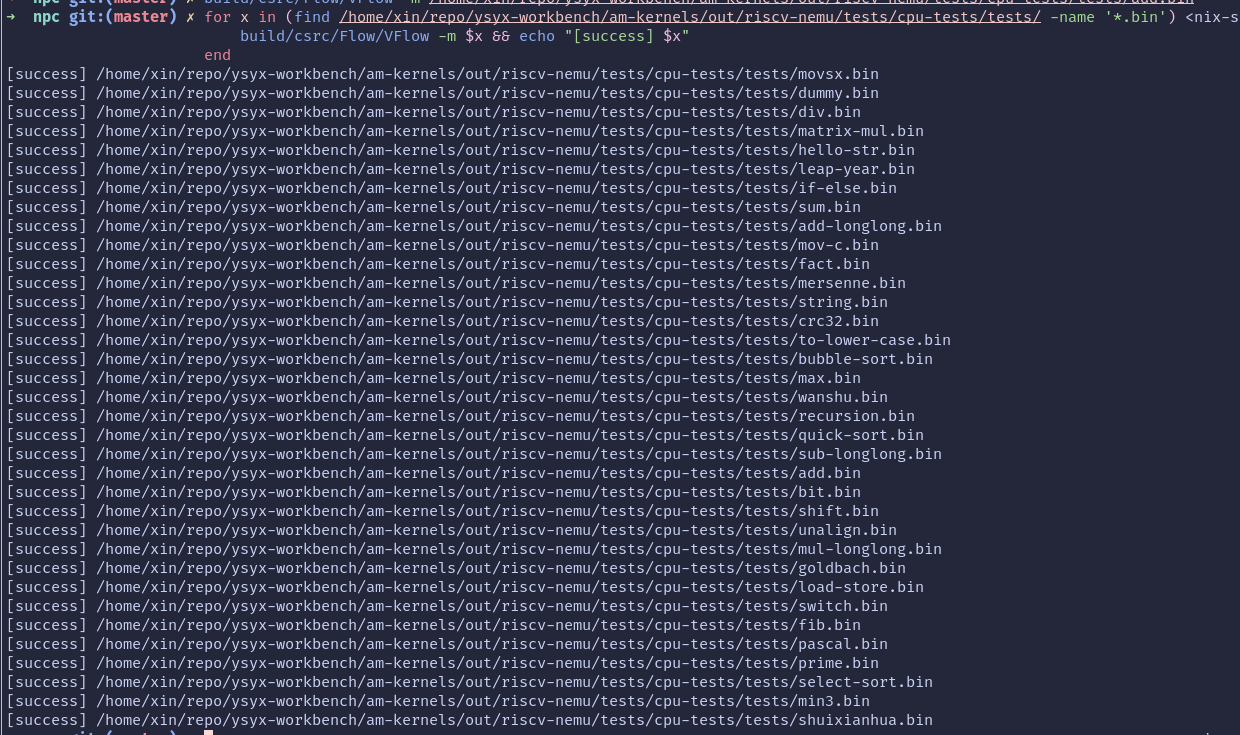
\includegraphics[width=\textwidth]{resources/test-cpu.png}
    \subcaption{cpu-tests测试结果}
    \label{fig:test-cpu}
\end{figure}

\begin{figure}
\centering

\begin{minipage}[t]{0.45\textwidth}
    \centering
    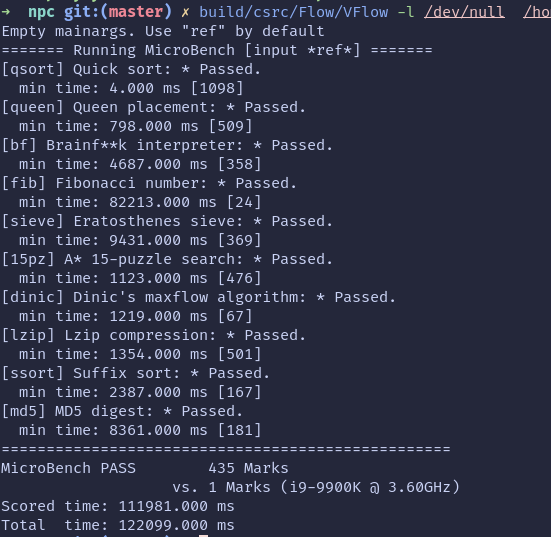
\includegraphics[width=\textwidth]{resources/test-bench.png}
    \subcaption{microbench测试结果}
    \label{fig:test-bench}
\end{minipage}
\begin{minipage}[t]{0.45\textwidth}
    \centering
    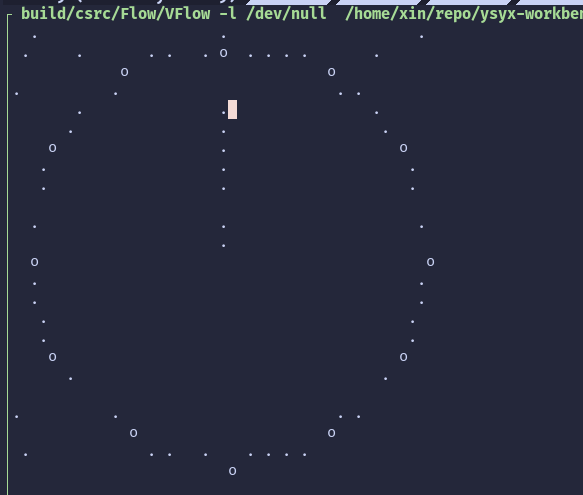
\includegraphics[width=\textwidth]{resources/test-clock.png}
    \subcaption{demo程序运行结果}
    \label{fig:2-machines-bm}
\end{minipage}
\caption{microbench和demo运行结果}
\end{figure}

\section{持续测试平台的搭建}

为了能够在芯片迭代的过程中持续对芯片的功能和性能进行测试,本文还搭建了持续测试平台。每次提交代码时,测试都会自动编译、测试,并报告可能发生的错误。

测试平台基于Gitea action搭建,可以离线部署,后续可以添加自动判分的功能,从而实现在课堂实验上使用。

\begin{figure}
    \centering
    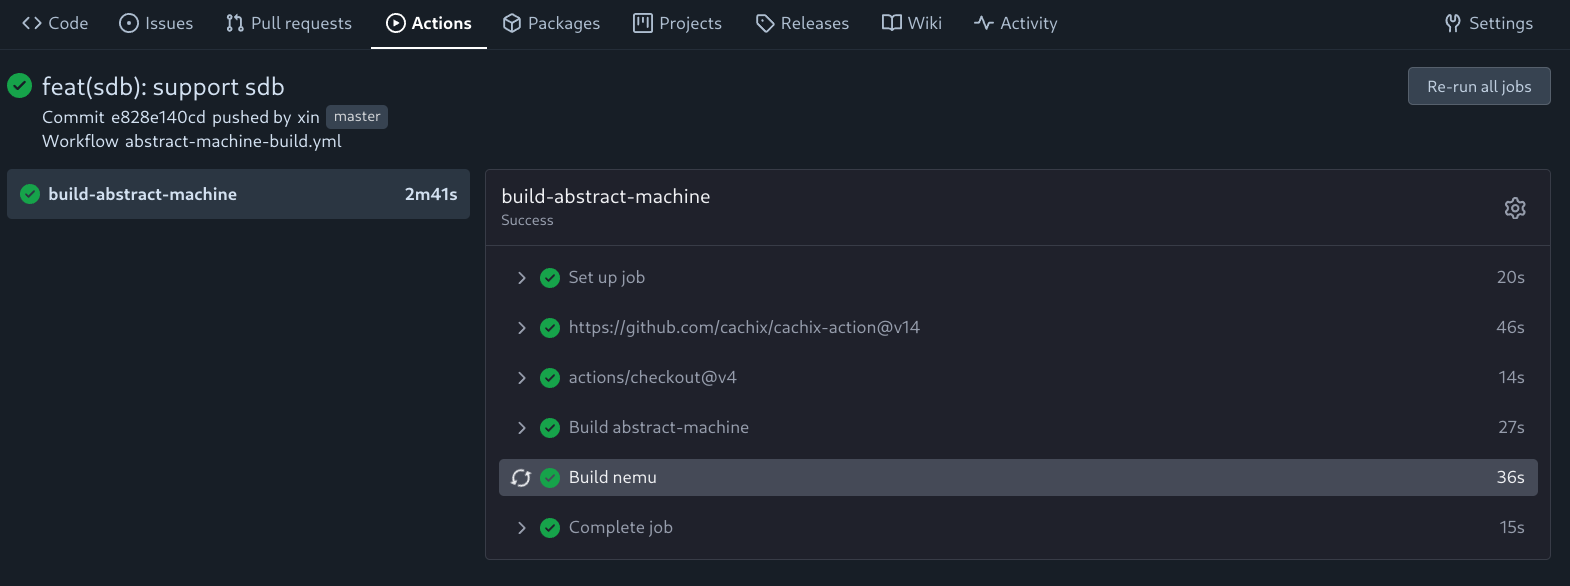
\includegraphics[width=0.8\textwidth]{resources/test-ci.png}
    \caption{持续测试平台运行}
    \label{fig:test-ci}
\end{figure}


\chapter{总结与展望}

\section{本文工作}

本文的主要贡献可以归结为以下两个方面:首先,本研究提出了一套针对芯片前期开发的可复用流程。该流程涵盖了从程序编译到仿真测试再到迭代优化的全过程,极大地提高了开发效率并减少了开发周期。其次,依托于该开发流程,本文使用Chisel语言设计并实现了一个基于四级流水线架构的RISC-V处理器。该处理器不仅支持基本的运算,还实现了简单的异常处理机制和总线接口,为处理更复杂的运算任务和系统扩展提供了可能。

为了提高芯片开发的效率和准确性,本研究基于NEMU模拟器和difftest差分测试工具,构建了一个可调试的芯片开发测试环境。该环境不仅支持详细的执行追踪和断点设置,还能实现自动化的错误检测,显著提高了开发流程的可靠性和工作效率。

进一步地,本文对abstract-machine进行了重要的改进。Abstract-machine原本是一个高度集成的硬件抽象层,用于简化硬件操作的复杂性。本研究对其进行了解耦和重构,将其打包为独立的软件库,便于第三方软件调用和集成。这一改动使得abstract-machine不仅在本项目中发挥了重要作用,也为其他研究者和开发者提供了一个可重用的、高效的硬件抽象接口。

另外,本文设计了一个四级流水线的处理器,详细介绍了处理器的每一个组成部分,包括指令解码、执行单元的设计以及流水线的控制逻辑。同时,本文还针对流水线设计中遇到的各种冒险进行了分析,并提出了相应的解决策略,为类似的芯片设计提供一定的参考。

\section{未来工作}

\subsection{处理器性能优化}

尽管已经实现了基本的流水线架构,但当前处理器的性能仍有待提升。未来工作将重点关注以下几个方面:

\begin{itemize}
    \item 通过引入指令缓存(I-cache)和数据缓存(D-cache),可以显著减少处理器访问主存储器的次数,从而减少延迟并提高指令执行速率。本文中处理器的取指和执行单元都要通过总线访问内存,假如内存的访问周期大于1时,流水线大多数时间都会处于阻塞状态。
    \item 增加转发单元,使其和计分板一同工作,从而减少非必要的数据冒险。通过设计高效的转发单元,可以直接从执行单元将数据转发到需要它的流水线阶段,而不必等待数据写回寄存器文件。
    \item 增加分支预测单元。分支指令的预测不准确会导致流水线的效率大幅下降,因为错误的预测需要撤销后续所有错误路径上的指令。通过引入一个高效的分支预测单元,可以提前正确预测程序的执行路径,从而减少因分支错误导致的处理器资源浪费。本文中固定取下一条指令的策略在遇到向前跳转的循环时,预测准确率非常低。
\end{itemize}

\subsection{FPGA验证}

目前处理器实现了AXI4-Lite总线协议的支持,未来将计划将其部署在FPGA上进行实际的硬件验证。这一步骤是验证处理器设计正确性及其性能的关键。通过FPGA验证,可以实际观察处理器在真实硬件条件下的运行状态和性能表现,及时发现设计上的不足,并对处理器设计进行必要的调整。此外,FPGA平台的使用还将为处理器与外部设备的交互提供实验环境,进一步验证系统的稳定性和可靠性。


\clearpage

\bibliography{ref/RISCV}

\include{pages/thanks}    % 致谢
\end{document}

